\chapter{Future Work}
Even though the estimation accuracy we achieved for DHI is acceptable for this application, but there is still room for improvement in some areas. For example, 
we know that different cloud types have different cloud-base-height as Figure \ref{fig:cloud_type} shows. They also have different reflection albedo and behavior of sunlight on each one is unique.Therefore, knowing which cloud type is dominant in the sky at each image can helps us to define better cloud segmentation strategies, classify the sun-state more accurately and finally estimate the diffuse irradiation with less error range. The approximated cloud-base-height from cloud type can also be used for projecting sun rays to the PV plant site in order to find correct shadow map which is very helpful when converting estimated total irradiation to power output.

\begin{figure}[h!]
\caption{Cloud types and their base-heights}
\label{fig:cloud_type}
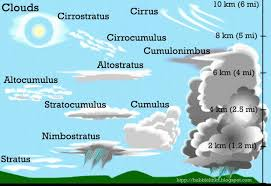
\includegraphics[scale=1]{cloud_types2}
\centering
\end{figure}

Another area for future work is sun-states. Since in this study we only used sun-states=1,4 there is still many images with sun-states of 2 and 3 which needs to be correctly handled in terms of effective DNI and DHI in them. Figure \ref{fig:img_state_2} shows examples of these images where sun is either visible behind a thin cloud for partically covered by a thick cloud respectively. Estimating DNI and DHI target values based on observed irradiances in sensor 1 (horizontal) and sensor 2 (titled) is another task which will help in this area.

\begin{figure}[h!]
\caption{An example of sun-state=2 (left) and sun-state=3 (right)}
\label{fig:img_state_2}
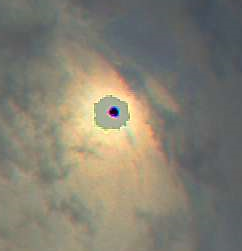
\includegraphics[scale=.5]{partial_opaque_sun}
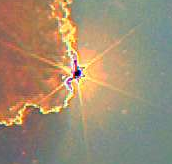
\includegraphics[scale=.75]{partial_occluded_sun}
\centering
\end{figure}


As it was mentioned in SVR result discussion, developing new derived features from the base features can help increase the correlation of features to the targets, thus improving the estimation accuracy. Finally, the reflection coming from surrounding structures such as mountains needs to investigated specifically in the morning and evening when these contributions seems to be more significant than other times of the day.